\section{Kernel step 5 Count changed word lanes rather than changed groups}
Fill \texttt{video\_group\_count}. Inspect each of the four word lanes in \texttt{\$w2}, form a zero/nonzero Boolean, and accumulate it in \texttt{\$v1}. An unsigned or signed word extraction can support this predicate because both preserve whether the word is zero. Treat a lane containing only bit 31 as nonzero.

For the worked group, two lanes are nonzero. At \texttt{video\_group\_counted}, the count is two while the pointers still name the original group. Adding one merely because the entire vector is nonzero would report one; counting nonzero bytes could report another value for a multibyte color change.

This simple lane extraction is a correct vector baseline. A later mask/reduction design may reduce the counting work, but it must count words under the same contract. Record that counting cost when comparing whole-kernel instruction counts.

\paragraph{Observe} Use \texttt{s05-1}; stop before \texttt{video\_group\_counted}. Inspect the state described above before continuing.

Figure~\ref{fig:video-vector-count} shows the same checkpoint in the source and debugger. Read the four bracketed values as words numbered zero through three from left to right. The value \texttt{0x88} has more than one set bit, but it still describes one changed word. Together with \texttt{0x10000}, it contributes two to the count.

% Native composition from verified, unchanged raw debugger captures.
\begin{figure}[htbp]
\centering
\sbox0{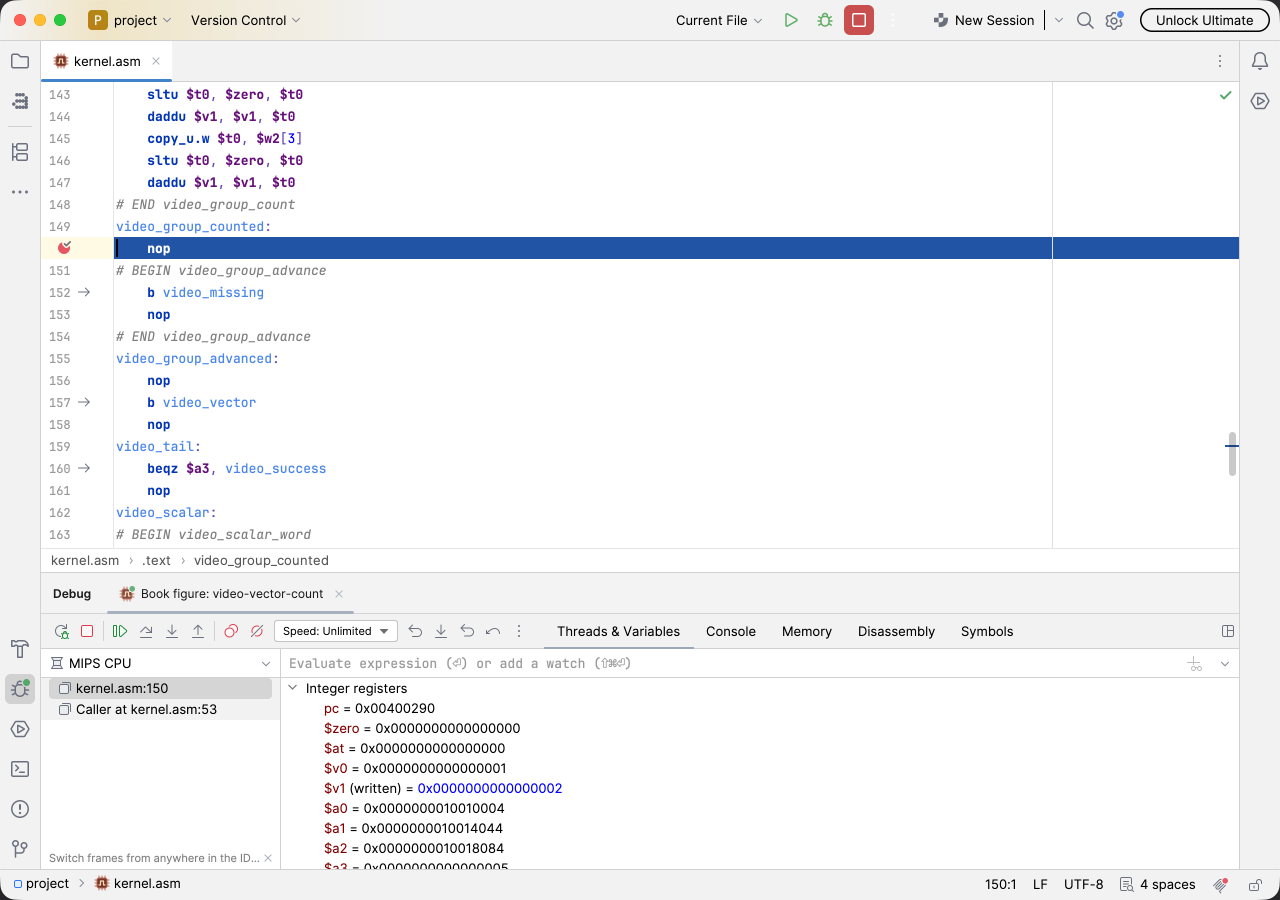
\includegraphics[artifact]{packages/034-lossless-video/captures/video-vector-count/counter.png}}
\sbox2{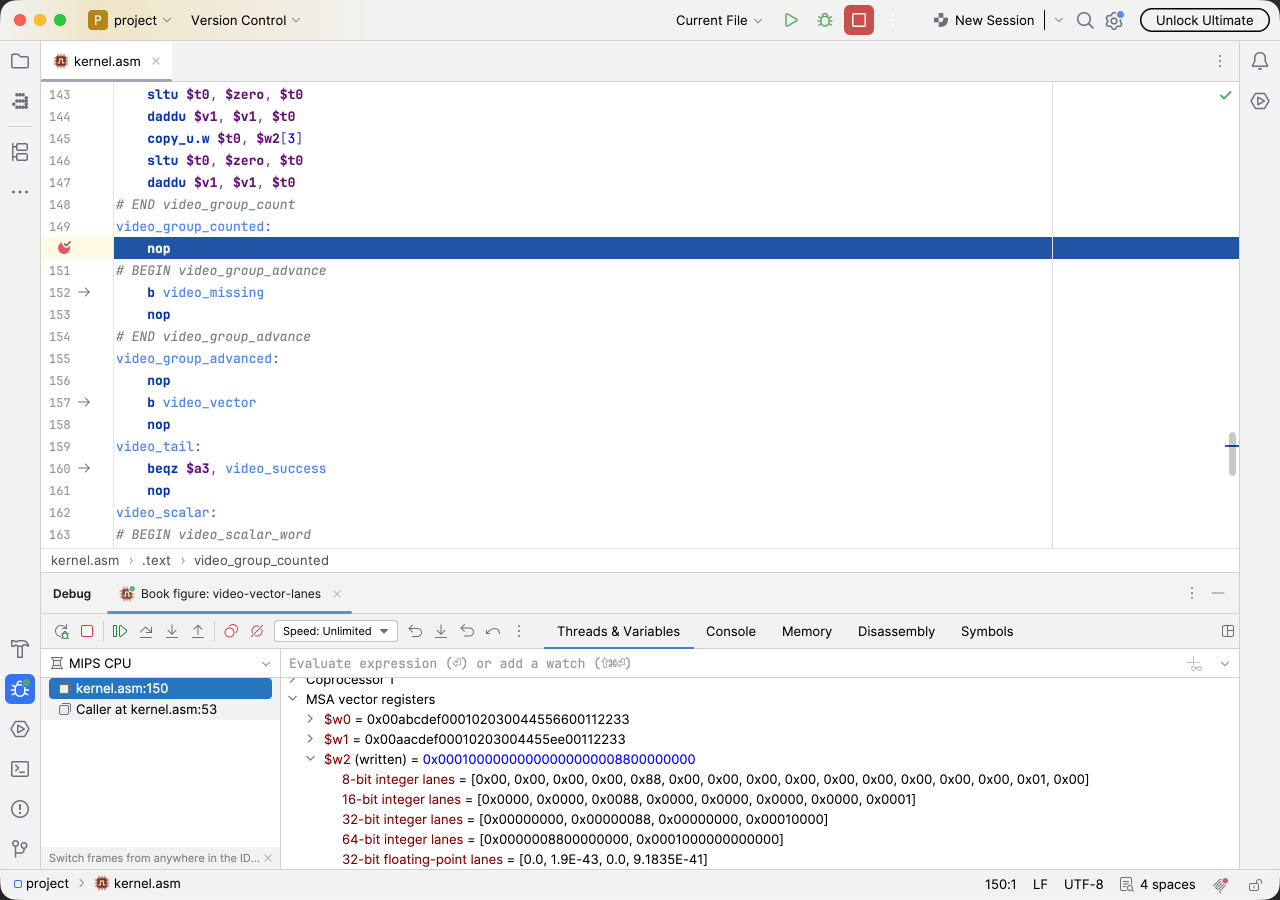
\includegraphics[artifact]{packages/034-lossless-video/captures/video-vector-count/lanes.png}}
\edef\MARSsourceLeft{\the\dimexpr0.031250000\wd0\relax}
\edef\MARSsourceBottom{\the\dimexpr0.710000000\ht0\relax}
\edef\MARSsourceRight{\the\dimexpr0.617187500\wd0\relax}
\edef\MARSsourceTop{\the\dimexpr0.236666667\ht0\relax}
\edef\MARSlanesLeft{\the\dimexpr0.257812500\wd2\relax}
\edef\MARSlanesBottom{\the\dimexpr0.078888889\ht2\relax}
\edef\MARSlanesRight{\the\dimexpr0.344531250\wd2\relax}
\edef\MARSlanesTop{\the\dimexpr0.898888889\ht2\relax}
\edef\MARScountLeft{\the\dimexpr0.246093750\wd0\relax}
\edef\MARScountBottom{\the\dimexpr0.113333333\ht0\relax}
\edef\MARScountRight{\the\dimexpr0.554687500\wd0\relax}
\edef\MARScountTop{\the\dimexpr0.864444444\ht0\relax}
\begin{tikzpicture}[alt={Three annotated debugger details at video_group_counted, before its nop. Callout 1 marks the next instruction. Callout 2 shows w2 as four 32-bit lanes, numbered zero through three from left to right: 0x00000000, 0x00000088, 0x00000000, 0x00010000. Only lanes one and three are nonzero. Callout 3 shows v1 equal to two. The next pointer-advance region is still unfinished.}]
\node[anchor=north west,inner sep=0,font=\small\bfseries] (source-title) at (6mm,0) {Paused source checkpoint};
\node[anchor=north west,inner sep=0] (source) at ([yshift=-2mm]source-title.south west) {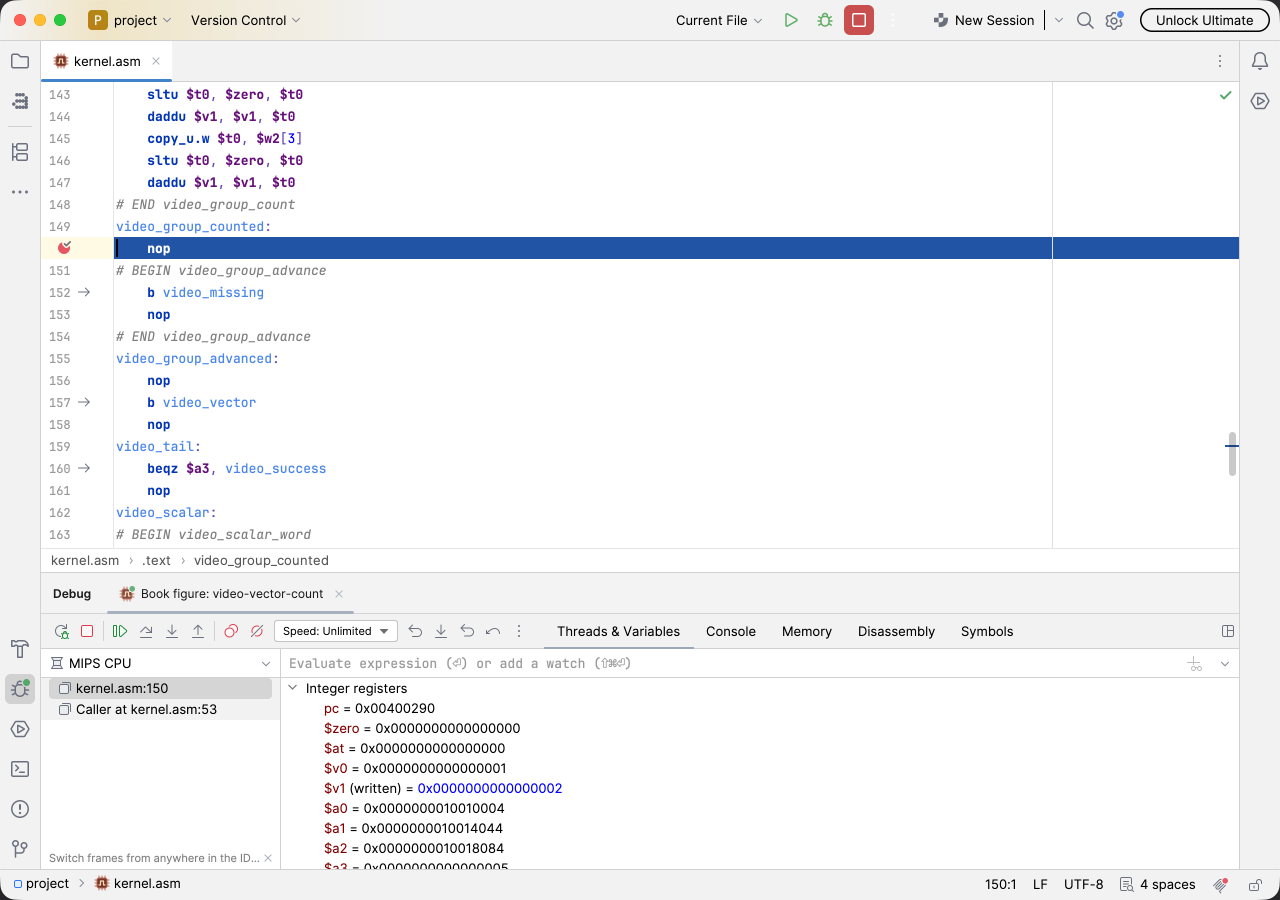
\includegraphics[width=0.75\linewidth,artifact,trim={\MARSsourceLeft{} \MARSsourceBottom{} \MARSsourceRight{} \MARSsourceTop{}},clip]{packages/034-lossless-video/captures/video-vector-count/counter.png}};
\begin{scope}[shift={(source.south west)},x={($(source.south east)-(source.south west)$)},y={($(source.north west)-(source.south west)$)}]
\draw[black,line width=0.7pt] (0.168888889,0.041666667) rectangle (0.288888889,0.500000000);
\node[draw=black,fill=white,circle,inner sep=1.5pt,font=\footnotesize] at ($(0.168888889,0.500000000)+(-3mm,0)$) {1};
\end{scope}
\node[anchor=north west,inner sep=0,font=\small\bfseries] (lanes-title) at ([yshift=-5mm]source.south west) {Four 32-bit word lanes};
\node[anchor=north west,inner sep=0] (lanes) at ([yshift=-2mm]lanes-title.south west) {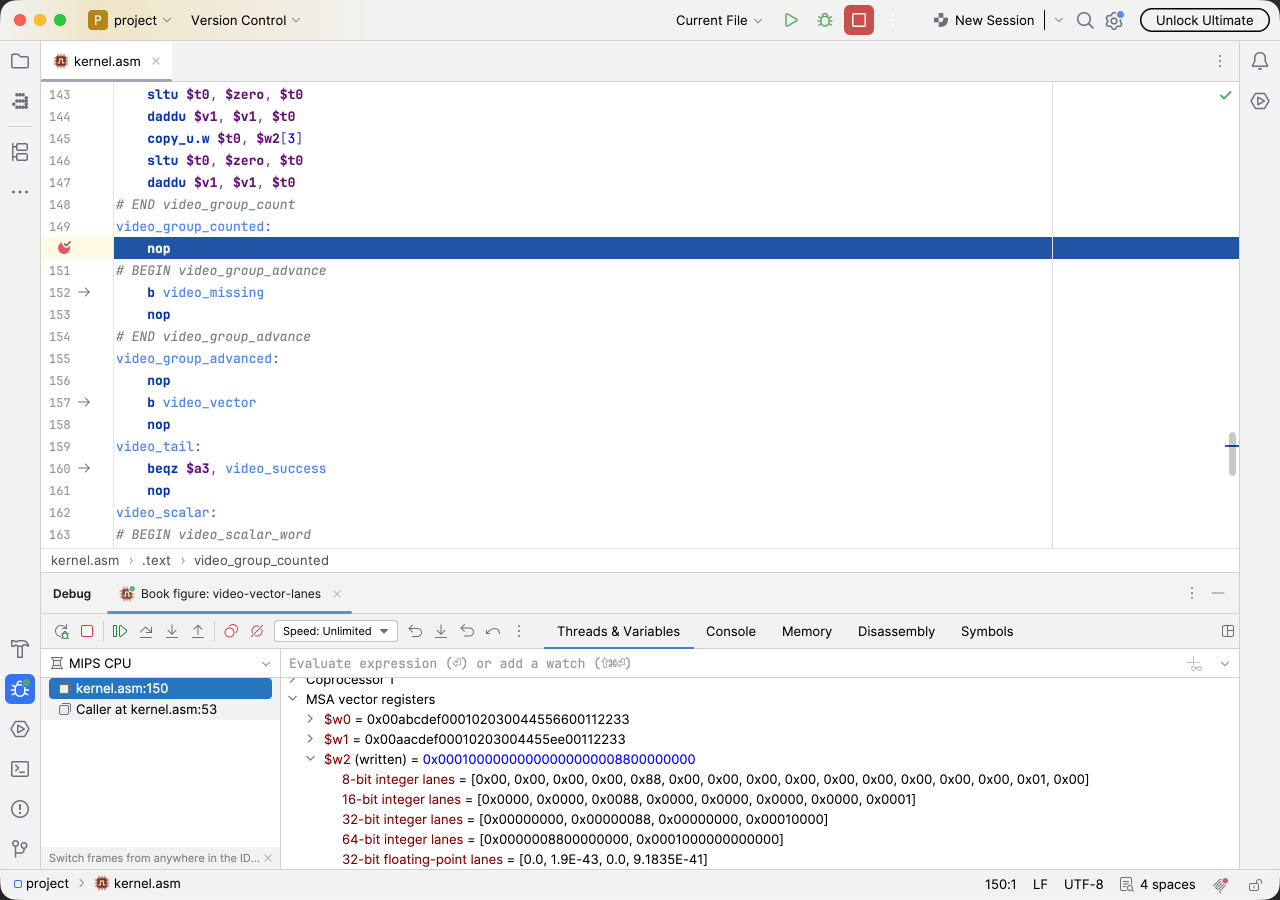
\includegraphics[width=\dimexpr\linewidth-6mm\relax,artifact,trim={\MARSlanesLeft{} \MARSlanesBottom{} \MARSlanesRight{} \MARSlanesTop{}},clip]{packages/034-lossless-video/captures/video-vector-count/lanes.png}};
\begin{scope}[shift={(lanes.south west)},x={($(lanes.south east)-(lanes.south west)$)},y={($(lanes.north west)-(lanes.south west)$)}]
\draw[black,line width=0.7pt] (0.017681729,0.000000000) rectangle (0.982318271,1.000000000);
\node[draw=black,fill=white,circle,inner sep=1.5pt,font=\footnotesize] at ($(0.017681729,1.000000000)+(-3mm,0)$) {2};
\end{scope}
\node[anchor=north west,inner sep=0,font=\small\bfseries] (count-title) at ([yshift=-5mm]lanes.south west) {Accumulated changed-word count};
\node[anchor=north west,inner sep=0] (count) at ([yshift=-2mm]count-title.south west) {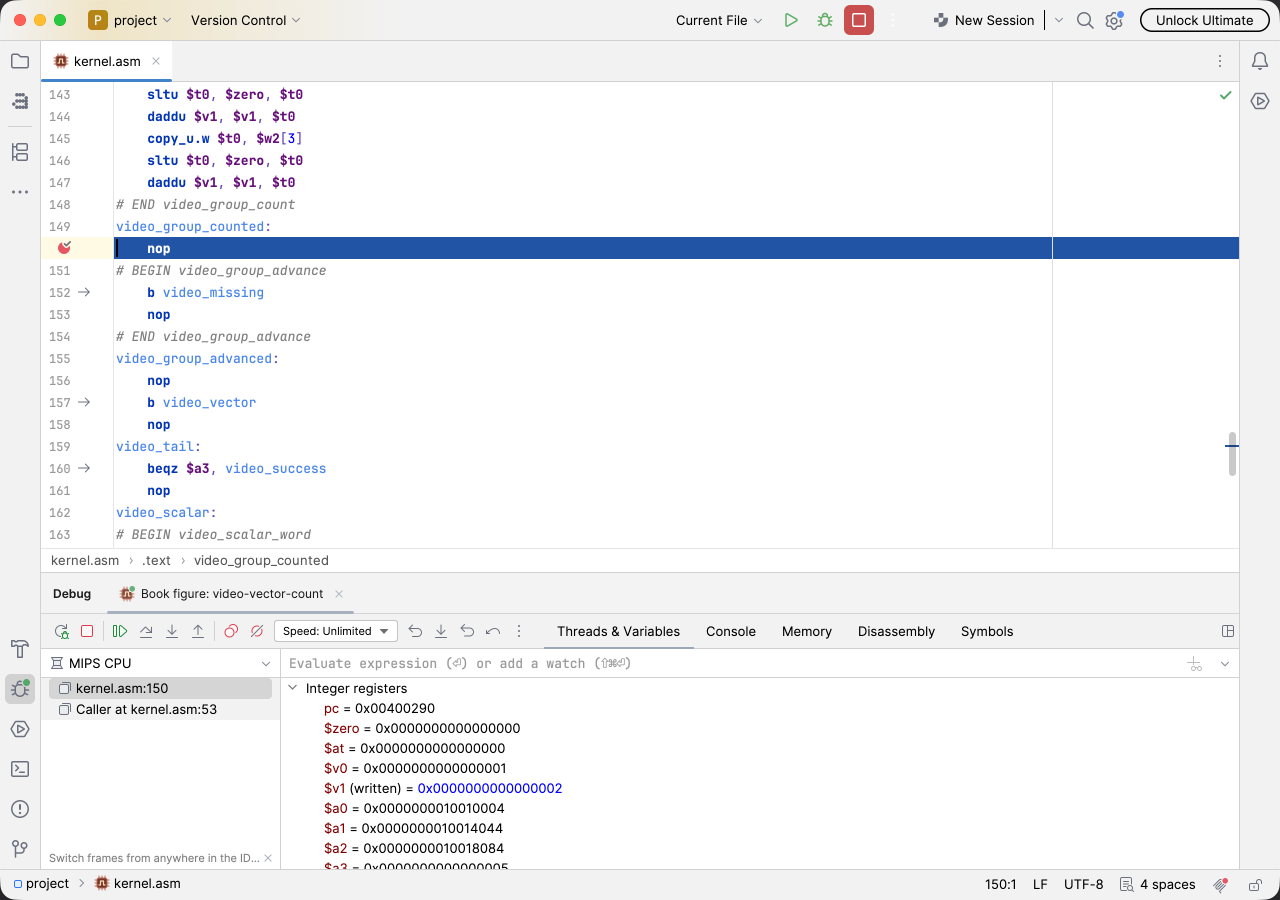
\includegraphics[width=0.52\linewidth,artifact,trim={\MARScountLeft{} \MARScountBottom{} \MARScountRight{} \MARScountTop{}},clip]{packages/034-lossless-video/captures/video-vector-count/counter.png}};
\begin{scope}[shift={(count.south west)},x={($(count.south east)-(count.south west)$)},y={($(count.north west)-(count.south west)$)}]
\draw[black,line width=0.7pt] (0.023529412,0.000000000) rectangle (0.976470588,1.000000000);
\node[draw=black,fill=white,circle,inner sep=1.5pt,font=\footnotesize] at ($(0.023529412,1.000000000)+(-3mm,0)$) {3};
\end{scope}
\end{tikzpicture}
\par\smallskip
\begin{minipage}{\linewidth}
\begin{enumerate}
\item The debugger is paused before the checkpoint \texttt{nop}. The next pointer-advance region is still unfinished.
\item Lane zero is on the left. Lanes one and three are nonzero; each contributes one changed word.
\item \texttt{\$v1} contains two, the number of changed words in this group.
\end{enumerate}
\end{minipage}
\caption{Word lanes and their changed-word count at the step-five checkpoint. The views come from two Debug launches with the same source and input.}
\label{fig:video-vector-count}
\end{figure}


\Needspace{7\baselineskip}
\paragraph{Check} How many changes does a group with two nonzero word lanes contribute?
\begin{itemize}
  \item[A.] One.
  \item[B.] Two.
  \item[C.] The number of nonzero bytes in those lanes.
\end{itemize}
